\section{Ход работы}

\subsection{Создание репозитория и фиксация начального состояния}

С помощью контекстного меню проводника Windows в рабочей папке проекта
\verb|BMSTU_IU5_MAGA_TERM1-TRPO-Lab1| запущен Git GUI, создан новый локальный
репозиторий. В каталог репозитория добавлен файл main.c с исходным кодом
программы, выводящей приветствие «Hello world!».
На рисунке~\ref{fig:file-1} показано состояние main.c до добавления в список на фиксацию.

\begin{figure}[htbp]
	\centering
	\reportScreenshot{figures/01-file.png}
	\caption{Файл main.c перед добавлением в фиксацию (Git GUI)}
	\label{fig:file-1}
\end{figure}

После подготовки файла и ввода комментария к фиксации выполнен первый commit
с сообщением «Initial commit». На рисунке~\ref{fig:init-commit} в окне gitk показана история
репозитория и содержимое зафиксированного изменения.

\begin{figure}[htbp]
	\centering
	\reportScreenshot{figures/02-init-commit.png}
	\caption{История после фиксации начального состояния (Initial commit)}
	\label{fig:init-commit}
\end{figure}

\subsection{Внесение изменений и повторная фиксация}

Программа доработана: вместо статического текста main.c
теперь запрашивает у пользователя имя (fgets) и выводит
персонализированное приветствие. Изменения проиндексированы
и зафиксированы отдельным коммитом «Give a personalized hello.».
На рисунке~\ref{fig:personalized-hello-commit} приведена фиксация данного изменения в gitk (показаны изменения в main.c).

\begin{figure}[htbp]
	\centering
	\reportScreenshot{figures/03-personalized-hello-commit.png}
	\caption{Фиксация изменения «Give a personalized hello»}
	\label{fig:personalized-hello-commit}
\end{figure}

\subsection{Планирование выпуска}

После подготовки Product Backlog было выполнено планирование первого выпуска.
В Jira выпуск представлен сущностью Release (Version), которая объединяет
сюжеты, планируемые к реализации к определенной дате. Для выпуска были заданы
начальная и конечная даты.

Владелец продукта определил, какие элементы из общей очереди должны войти в
первый выпуск. Для выбранных сюжетов была установлена соответствующая версия
выпуска. При этом часть требований могла оставаться только в Product Backlog и
не включаться в текущий выпуск. Такое разделение позволяет отличать весь объем
потенциальной работы над продуктом от обязательств, принятых на конкретный
выпуск. Результат планирования показан на рисунке~\ref{fig:release}.

\begin{figure}[htbp]
	\centering
	\reportScreenshot{figures/05-release.png}
	\caption{Планирование выпуска 1.0}
	\label{fig:release}
\end{figure}

\subsection{Планирование спринта}

После определения состава выпуска было выполнено планирование первого спринта.
На этом этапе основную организационную роль выполнял Scrum Master,
а решение о фактически принимаемом объеме работы
принималось совместно с командой. Владелец продукта пояснял приоритеты и
требования, участники команды оценивали реализуемость выбранного объема работ.

Из очереди выпуска в первый спринт было перенесено тир истории.
Для спринта была определена цель, отражающая
результат, который команда должна получить к окончанию итерации. Также был
подготовлен следующий спринт, который впоследствии используется для переноса
незавершенной работы. Сформированный Sprint Backlog представлен на
рисунке~\ref{fig:sprint}.

\begin{figure}[htbp]
	\centering
	\reportScreenshot{figures/06-sprint.png}
	\caption{Планирование первого спринта}
	\label{fig:sprint}
\end{figure}

\subsection{Декомпозиция, оценка и распределение заданий}

Каждый сюжет, включенный в первый спринт, был декомпозирован на более мелкие
технические задания.

Сюжеты и технические задания оценивались по-разному. Сложность Story была ранее
выражена в Story Points, тогда как для Sub-task задавалась временная оценка в
часах. После оценки задачи были распределены между непосредственными
исполнителями. При этом сюжеты оставались элементами верхнего уровня, а
исполнители назначались прежде всего на конкретные технические задачи. При
распределении учитывалась суммарная загрузка участников, чтобы избежать
существенного дисбаланса работы внутри спринта. Результат декомпозиции и
назначения заданий приведен на рисунке~\ref{fig:tasks}.

\begin{figure}[htbp]
	\centering
	\reportScreenshot{figures/07-tasks.png}
	\caption{Декомпозиция и распределение заданий первого спринта}
	\label{fig:tasks}
\end{figure}

\subsection{Просмотр и выполнение заданий}

После запуска спринта участники команды перешли к выполнению назначенных задач.
Для оперативной работы использовалась Scrum-доска со статусами, соответствующими
основным состояниям задания: \textit{To Do}, \textit{In Progress} и
\textit{Done}. При начале работы задача переводилась в состояние выполнения, а
после завершения --- в состояние готовности.

В ходе работы участники актуализировали сведения о задачах: фиксировали
выполненную работу, при необходимости корректировали оставшуюся оценку и
добавляли комментарии о текущем состоянии. Это позволяет Scrum Master и другим
участникам команды видеть не только формальный статус рабочего элемента, но и
фактический прогресс по нему. Завершение дочерних задач служило основанием для
проверки и последующего завершения родительского сюжета.

\subsection{Отслеживание хода работы}

Контроль выполнения спринта осуществлялся Scrum Master. Для этого использовались
возможности поиска и фильтрации рабочих элементов Jira, являющиеся аналогом
запросов IBM Team Concert. Были рассмотрены выборки, позволяющие отдельно
контролировать элементы Product Backlog, работы текущего выпуска, задачи первого
спринта, недавно измененные элементы и незавершенную работу.

Дополнительно состояние итерации контролировалось по встроенным отчетам Jira.
Отчет Burndown позволяет сравнивать оставшийся объем работы с ожидаемой динамикой
его уменьшения к окончанию спринта. Для контроля выпуска использовалась
агрегированная информация по элементам, связанным с Release 1.0. Также сведения о
состоянии проекта могут быть вынесены на Dashboard, что обеспечивает быстрый
доступ к основным показателям проекта. Пример используемых средств контроля
представлен на рисунке~\ref{fig:tracking}.

\begin{figure}[htbp]
	\centering
	\reportScreenshot{figures/08-tracking.png}
	\caption{Отслеживание хода выполнения работ}
	\label{fig:tracking}
\end{figure}

\subsection{Проверка результатов спринта}

По завершении основной части работ была проведена проверка результатов спринта
(Sprint Review). Ее назначение состоит в демонстрации полученного инкремента
заинтересованным лицам и получении обратной связи. В ходе проверки участники
команды демонстрируют завершенную функциональность, а владелец продукта оценивает
результат с точки зрения требований и целей спринта.

Полученные замечания и предложения были зафиксированы для использования в
дальнейшем планировании. В Jira для хранения результатов проверки может
использоваться отдельный рабочий элемент либо описание и комментарии, связанные
со спринтом. Подготовка и фиксация результатов проверки показаны на
рисунке~\ref{fig:review}.

\begin{figure}[H]
	\centering
	\reportScreenshot{figures/09-review.png}
	\caption{Фиксация результатов проверки первого спринта}
	\label{fig:review}
\end{figure}

\subsection{Проведение ретроспективы}

После Sprint Review была проведена ретроспектива. В отличие от проверки
результата продукта, ретроспектива направлена на анализ процесса работы команды.
Участники обсудили, какие решения и организационные практики оказались удачными,
какие затруднения возникли в ходе итерации и что необходимо изменить в следующем
спринте.

Результатом ретроспективы стал набор конкретных выводов для следующей итерации:
уточнять критерии приемки до начала реализации, декомпозировать крупные задачи,
сохранять резерв времени и актуализировать оценки по мере выполнения работы.
Таким образом, ретроспектива завершила цикл обратной связи не только по продукту,
но и по процессу разработки.

\subsection{Закрытие спринта и подготовка следующей итерации}

Перед закрытием первого спринта было проверено состояние всех входящих в него
сюжетов и задач. Завершенные элементы были оставлены в составе закрываемой
итерации, а незавершенные рабочие элементы перенесены в следующий спринт. При
переносе учитывались как родительские сюжеты, так и относящиеся к ним дочерние
задачи, чтобы сохранить согласованность Sprint Backlog.

После этого первый спринт был завершен, а второй подготовлен к дальнейшему
планированию. В новую итерацию могут быть включены как перенесенные незавершенные
работы, так и новые сюжеты из очереди выпуска. Тем самым был воспроизведен полный
Scrum-цикл: от формирования Product Backlog и планирования выпуска до выполнения,
контроля, проверки, ретроспективы и перехода к следующей итерации. Результат
закрытия первого спринта показан на рисунке~\ref{fig:sprint-closed}.

\begin{figure}[H]
	\centering
	\reportScreenshot{figures/10-sprint-closed.png}
	\caption{Закрытие первого спринта и переход к следующей итерации}
	\label{fig:sprint-closed}
\end{figure}

\subsection{Формирование сводной панели}

Для централизованного контроля состояния проекта была настроена сводная
панель Jira. На ней были размещены виджеты, отображающие текущее состояние
задач и ход выполнения спринта. Использование сводной панели позволяет
получить обобщённое представление о состоянии проекта без необходимости
последовательного просмотра отдельных задач и отчётов.

Итоговый вид сводной панели проекта представлен на рисунке~\ref{fig:dashboard}.

\begin{figure}[H]
	\centering
	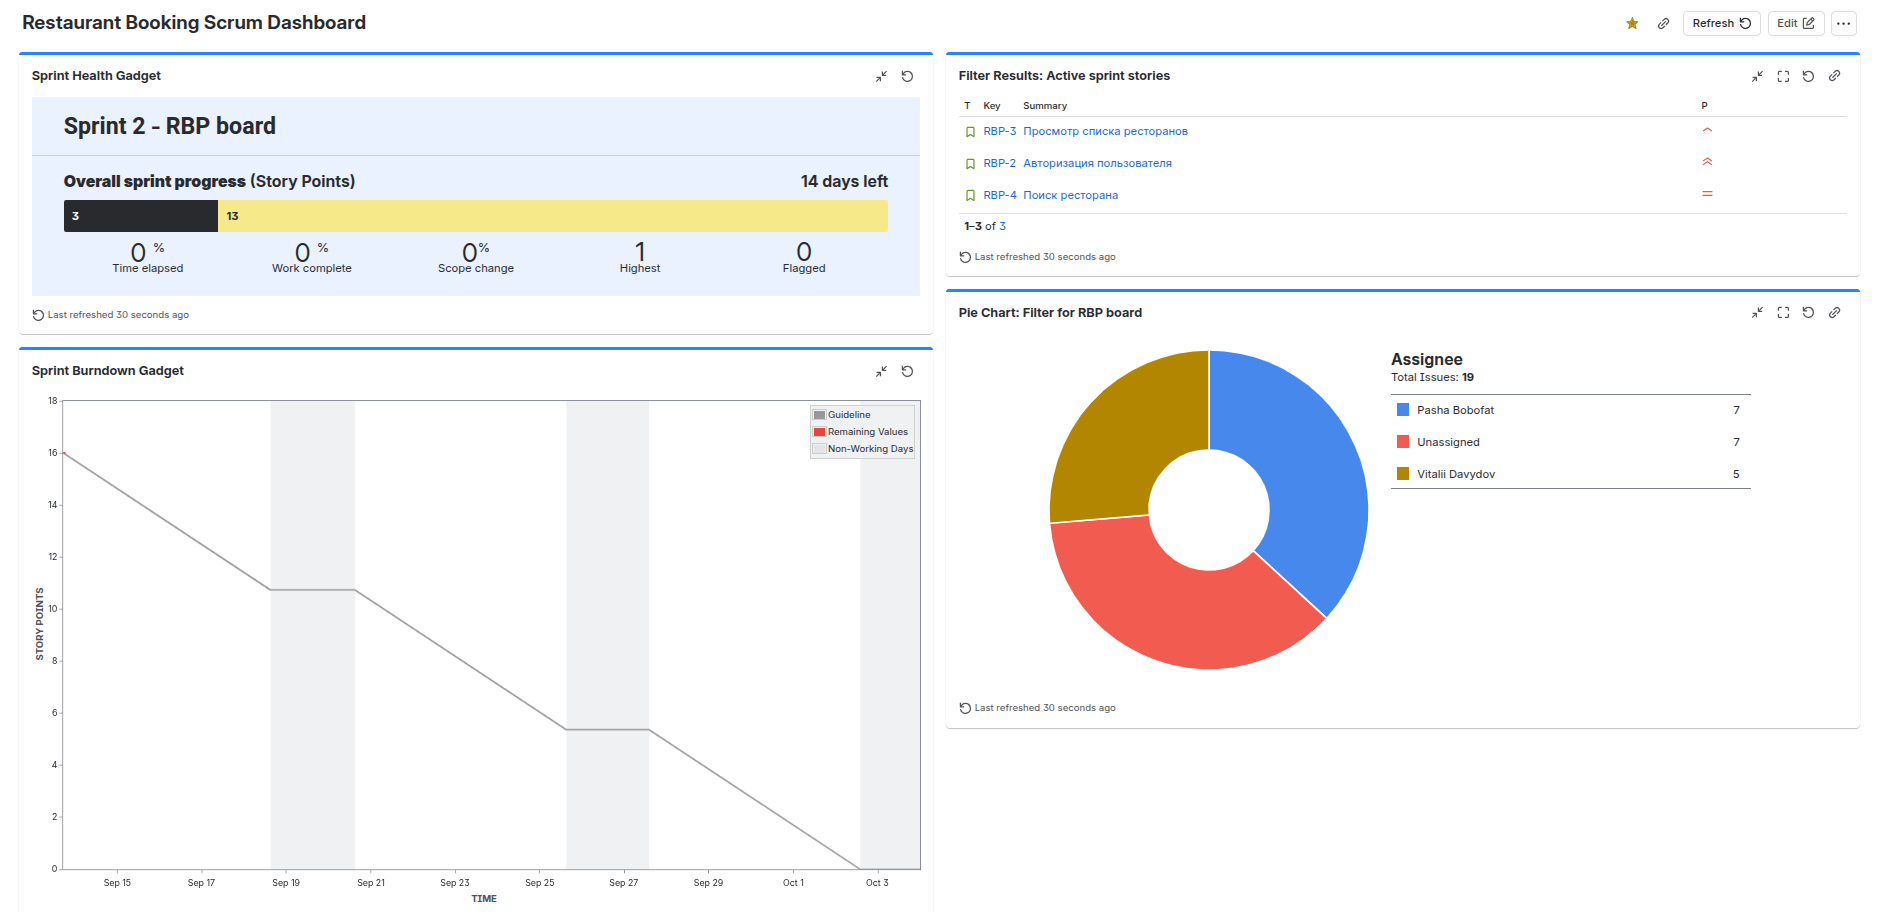
\includegraphics[width=\textwidth]{figures/11-dashboard.png}
	\caption{Сводная панель проекта}
	\label{fig:dashboard}
\end{figure}
